% Generated by worked_3d.py from the separate input table.
\begin{center}\small
\begin{tabular}{ll}
\hline
Illustrative input & Value\\
\hline
Mass $m$ & $2\,{\rm kg}$\\
Half extents $(a,b,c)$ & $(.20,.15,.10)\,{\rm m}$\\
Reference length $\ell$ & $.20\,{\rm m}$ (coordinate choice)\\
Incoming $\mathbf v^-$ & $(1,-.6,-2)\,{\rm m/s}$\\
Incoming $\boldsymbol\omega^-$ & $(2,-1,3)\,{\rm rad/s}$\\
Normal $\mathbf n$; tangents $\mathbf t_1,\mathbf t_2$ & $\mathbf e_z;\mathbf e_x,\mathbf e_y$\\
Normal restitution $e_n$ & $.6$\\
Tangential restitution $e_t$ & $.3$\\
Pair friction $\mu$ & $.6$\\
Boundary & Stationary plane, $z=0$\\
\hline
\end{tabular}\end{center}
These are prescribed illustration inputs, not a published material profile or fitted experimental values. The matrix equations below retain symbolic material coefficients. Attitude and lever-arm signs are fixed by the actual box geometry.
\begin{equation}
\mathbf A=\frac19\begin{bmatrix}1&4&8\\4&7&-4\\-8&4&-1\end{bmatrix},\qquad
\mathbf r_{\rm shape}=\begin{bmatrix}a\\-b\\c\end{bmatrix},\qquad
\mathbf r=\mathbf A\mathbf r_{\rm shape}.
\end{equation}
The supporting vertex is unique: every other vertex lies above the plane when the centre of mass is placed at $-\mathbf r$. For a homogeneous cuboid,
\begin{equation}
\mathbf I_{\rm shape}=\frac m3\operatorname{diag}(b^2+c^2,a^2+c^2,a^2+b^2),\qquad
\mathbf I=\mathbf A\mathbf I_{\rm shape}\mathbf A^T.
\end{equation}
\begin{equation}
\mathbf r=\begin{bmatrix}0.044444\\-0.072222\\-0.255556\end{bmatrix}\,{\rm m},\qquad
\mathbf I=\begin{bmatrix}0.039774 & -0.003868 & 0.000329\\-0.003868 & 0.032675 & 0.005021\\0.000329 & 0.005021 & 0.024218\end{bmatrix}\,{\rm kg\,m^2}.
\end{equation}
All three spin components are retained. The six-component state, mass block and three-by-six contact map are
\begin{equation}
\mathbf V^-=\begin{bmatrix}\mathbf v^-\\\ell\boldsymbol\omega^-\end{bmatrix},\qquad
\mathbf M=\begin{bmatrix}m\mathbf1_3&0\\0&\mathbf I/\ell^2\end{bmatrix},\qquad
\mathbf C=[\mathbf1_3\ \mathbf R].
\end{equation}
\begin{equation}
\mathbf R=\begin{bmatrix}-0.000000 & -1.277778 & 0.361111\\1.277778 & -0.000000 & 0.222222\\-0.361111 & -0.222222 & -0.000000\end{bmatrix},\qquad\mathbf u^-=\mathbf C\mathbf V^-.
\end{equation}
The stationary plane contributes zero inverse mass. Use the full tensor, then rotate into the ordered contact basis $(n,t_1,t_2)$:
\begin{equation}
\mathbf W=\mathbf C\mathbf M^{-1}\mathbf C^T,\qquad
\widehat{\mathbf W}=\mathbf Q^T\mathbf W\mathbf Q,\qquad
\mathbf Q=[\mathbf e_z\ \mathbf e_x\ \mathbf e_y].
\end{equation}
\begin{equation}
\widehat{\mathbf W}=\begin{bmatrix}0.716353 & 0.448661 & -0.489459\\0.448661 & 3.059430 & -0.012536\\-0.489459 & -0.012536 & 2.224217\end{bmatrix}\,{\rm kg^{-1}}.
\end{equation}
Its off-diagonal entries couple normal and tangential impulses: solving only its diagonal would give a different collision. Solve the small symmetric system rather than form an explicit inverse:
\begin{align}
\widehat{\mathbf W}\widehat{\mathbf j}+(\mathbf1+\mathbf E)\mathbf Q^T\mathbf u^-&=0,\qquad
\mathbf E=\operatorname{diag}(e_n,e_t,e_t),\\
\mathbf j&=\mathbf Q\widehat{\mathbf j},\\
\mathbf V^+&=\mathbf V^-+\mathbf M^{-1}\mathbf C^T\mathbf j.
\end{align}
Check $j_n\ge0$, $\|\mathbf j_t\|\le\mu j_n$ and the actual kinetic-energy increment before accepting that endpoint solution. Here the unconstrained target is admissible, so no friction-capacity adjustment is required.
\begin{center}\small
\begin{tabular}{ll}
\hline
Computed result & Value\\
\hline
$\mathbf u^-$, world $(x,y,z)$ & $(1.472222,0.044444,-2.100000)\,{\rm m/s}$\\
$\widehat{\mathbf j}$, contact $(n,t_1,t_2)$ & $(6.670214,-1.597877,1.432858)\,{\rm kg\,m/s}$\\
$\mathbf v^+$ & $(0.201062,0.116429,1.335107)\,{\rm m/s}$\\
$\boldsymbol\omega^+$ & $(-0.535728,2.560464,0.160786)\,{\rm rad/s}$\\
$\mathbf u^+$, world $(x,y,z)$ & $(-0.441667,-0.013333,1.260000)\,{\rm m/s}$\\
$\|\mathbf j_t\|/j_n$ & $0.321763$\\
$T^-$; $T^+$ & $5.559516$; $1.956965\,{\rm J}$\\
\hline
\end{tabular}\end{center}
The example changes translation and all three spin components while satisfying both restitution targets. Energy decreases; the stationary plane receives the opposing impulse. Linear and angular momentum are checked through their impulse balances, rather than assuming conservation for the cuboid alone.

The retained calculation compares scaled matrix operations with independent unscaled cross-product updates, checks the impulse/energy identities and the supporting vertex, and repeats the solve at four reference lengths and three rotated tangent bases. Physical impulses and outgoing states remain unchanged to the reported numerical precision. These are algebra and geometry checks, not an experimental accuracy claim or a native time-step replay.
\begin{figure}[htbp]
\centering
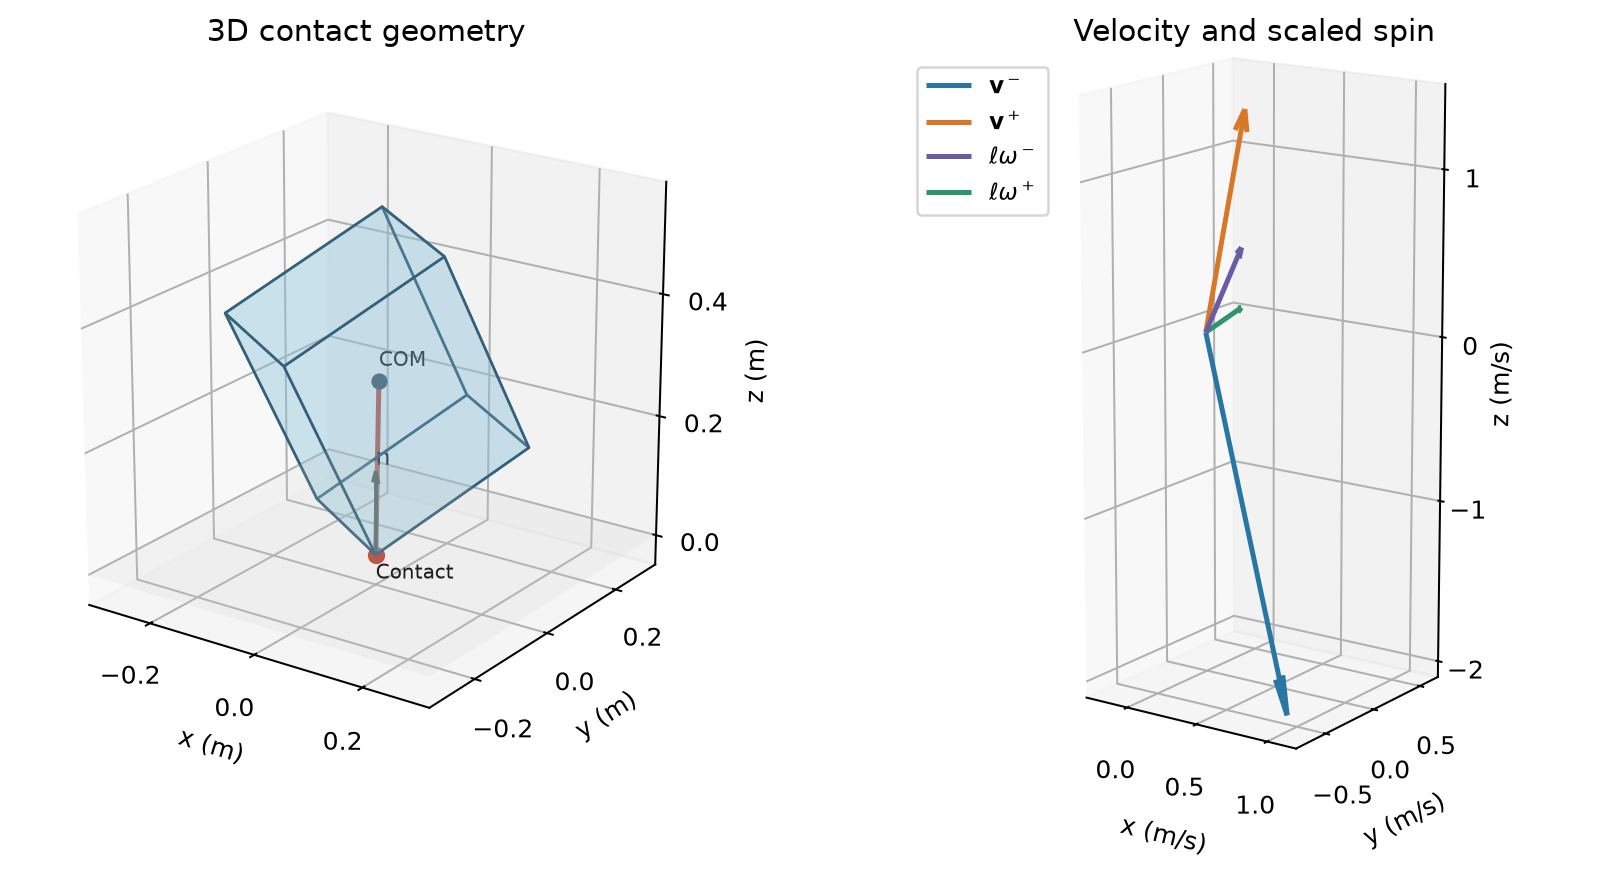
\includegraphics[width=\linewidth]{worked-3d-v1/geometry-motion.png}
\caption{The rotated cuboid contacts the plane at its unique lowest corner. The right panel compares incoming and outgoing translation and length-scaled spin in the same velocity units; arrows begin at a common origin for comparison. The impulse acts at the corner, while spin is defined about the centre of mass.}
\end{figure}
